\subsection*{Dufu is very busy}

\textit{Du Fu} (712-770) (en chinois \zh{杜甫} est un poète chinois de la dynastie Tang, célèbre pour sa prose teintée de réalisme où se croise scènettes de la vie quotidienne et descriptions des arcanes du pouvoir. Le mème ``Du Fu est vraiment très occupé'' \zh{杜甫很忙} détourne une calligraphie bien connue pour mettre en scène le poète dans des situations improbables : 

Voir la page sur \textit{Know Your Meme} :
\url{http://knowyourmeme.com/memes/du-fu-is-busy}
et sur l'encyclopédie Baidu
\url{http://wenku.baidu.com/view/941e25c805087632311212aa.html}

\begin{figure}[ht]
    \centering
    \subfloat[]{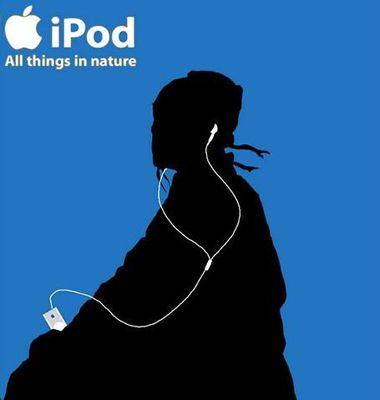
\includegraphics[scale=.4]{figures/annexes/dufu/8c7.jpg}}
    \subfloat[]{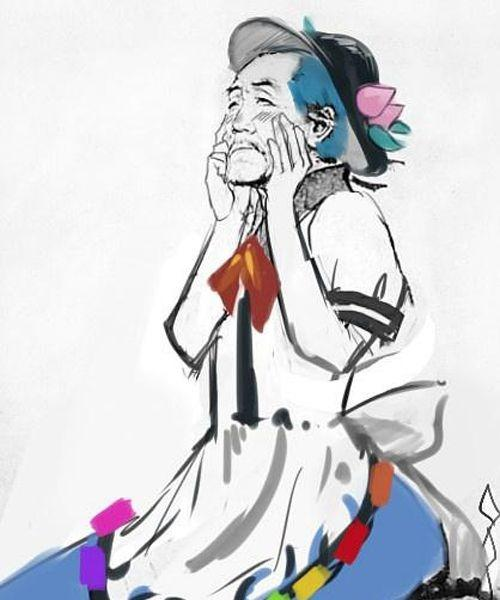
\includegraphics[scale=.3]{figures/annexes/dufu/8dd.jpg}}
    \subfloat[]{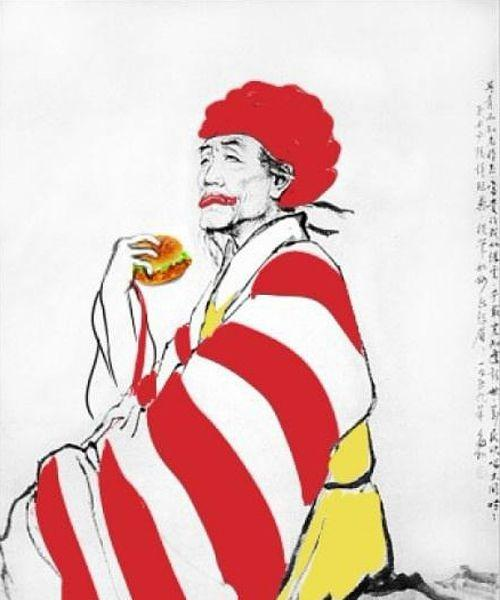
\includegraphics[scale=.3]{figures/annexes/dufu/b5f.jpg}}
    \newline
    \subfloat[]{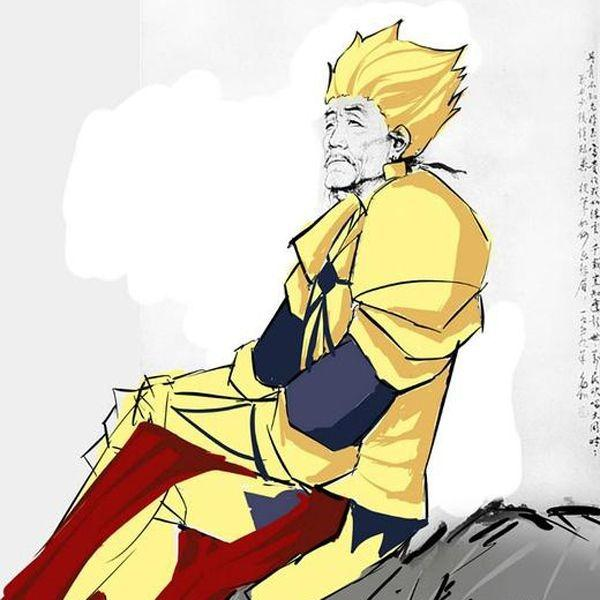
\includegraphics[scale=.3]{figures/annexes/dufu/bb3.jpg}}
    \subfloat[]{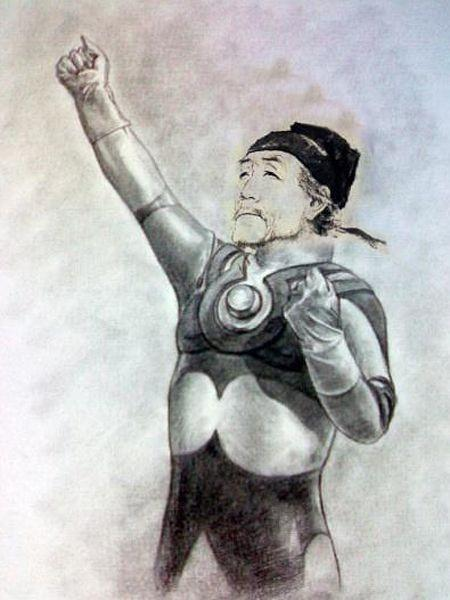
\includegraphics[scale=.3]{figures/annexes/dufu/bd8.jpg}}
    \subfloat[]{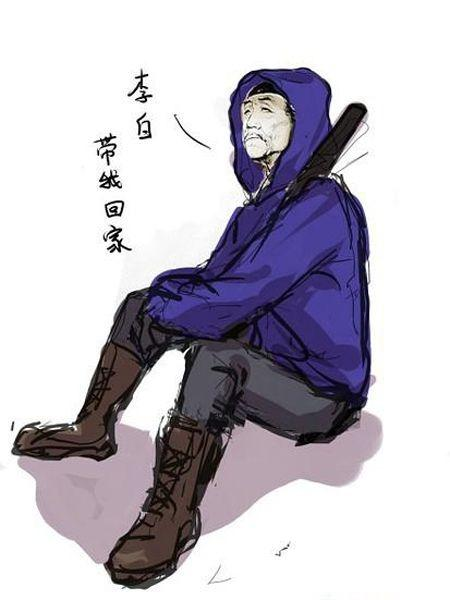
\includegraphics[scale=.3]{figures/annexes/dufu/d09.jpg}}
    \caption{
      Dufu is very busy 
    }
\end{figure}

\clearpage
\subsection*{The Voice of China}

\textit{The Voice of China} (en chinois \zh{中国好声音}) lest une émission de télé-crochet musical, diffusée en Chine depuis le 13 juin 2012 sur \textit{Zhejiang Television}. \textit{The Voice of China} est une adaptation de l'émission \textit{The Voice of Holland}, dont les droits ont été vendues dans le monde entier. Un jury composé de membres de l'industrie musicale chinoise prend part à l'émission afin de les juger l'interprétation de chansons populaires par des candidats choisis sur casting . Diffusés depuis Juillet 2012, les épisodes sont visionnés en moyenne par 7 millions de téléspectateurs et plus de 70 millions d'internautes (d'après Laurie Burkitt, ``Why The Voice Is China's No. 1 TV Show'' in \textit{The Wall Street Journal} du 19/09/2013)

Voir la page officielle : \url{http://www.zjstv.com/voice/}

\begin{figure}[htbp!]
    \centering
    \subfloat[Logo Officiel de The Voice of China]{
\includegraphics[scale=.47]{figures/annexes/thevoice/The_Voice_of_China_-_official_logo.jpg}}
    \subfloat[Les membres du Jury de l'édition 2014]{
\includegraphics[scale=.5]{figures/annexes/thevoice/The_Voice_of_China_S2.jpg}}
    \newline
    \subfloat[``The Voice devient le sujet le plus discuté du mois de Juillet'', d'après Hi News, \url{http://www.hinews.cn/news/system/2012/08/25/014863154.shtml}, consulté le 7 Juillet à 14:32]{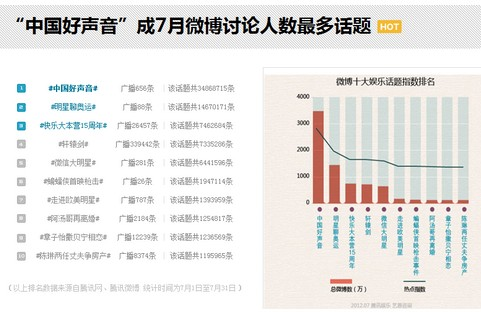
\includegraphics[scale=.8]{figures/annexes/thevoice/weibo-trends.jpg}}
    \subfloat[Un dessin posté par un utilisateur de Sina Weibo]{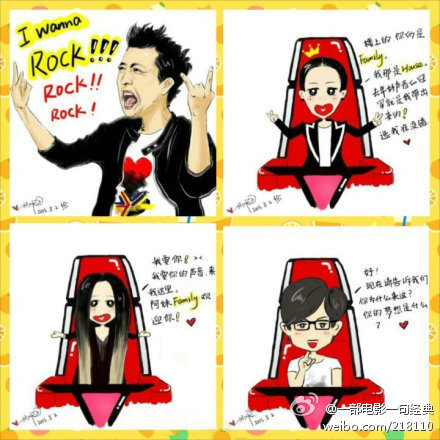
\includegraphics[scale=.42]{figures/annexes/thevoice/7ff5fbaftw1e7ilgxti2bj20c80c8gn2.jpg}}
    \caption{
      The Voice of China : Illustrations
    }
\end{figure}

\clearpage
\subsection*{Biaoge}
\label{sec:biaoge}

En Août 2012, Yang Dacai, directeur du Bureau de Supervision de la Sécurité Routière de la province du Shanxi, se rend sur les lieux d'un accident de bus ayant fait 36 morts. Une photo diffusée sur Internet le montre discutant avec un policier, arborant un grand sourire. Agacé par cette excès d'incivilité, les internautes commencent à faire des recherches à son sujet et se rendent compte que l'officiel chinois arborent à chaque apparition une montre différente, toutes de marques prestigieuses. Les internautes le renomment rapidement \textit{le frère aux montres} (\textit{biaoge}) et collectent les photos de ses différentes montres de luxe comme autant de preuves manifestes de sa corruption. Quelques jours plus tard, Yang Dacai est démis de ces fonctions. Il sera par la suite jugé et condamné pour corruption, assorti d'une peine de 12 ans de prison. 

Voir aussi : \url{http://www.scmp.com/topics/yang-dacai} ou \url{http://www.chinasmack.com/2012/pictures/chinese-government-official-smiling-at-tragic-accident-scene.html}

\begin{figure}[h!]
    \centering
    \subfloat[]{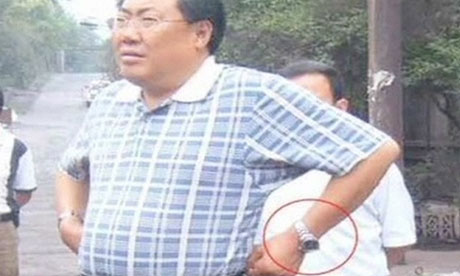
\includegraphics[scale=.5]{figures/annexes/biaoge/Yang-Dacai-wearing-one-of-010.jpg}}
    \subfloat[]{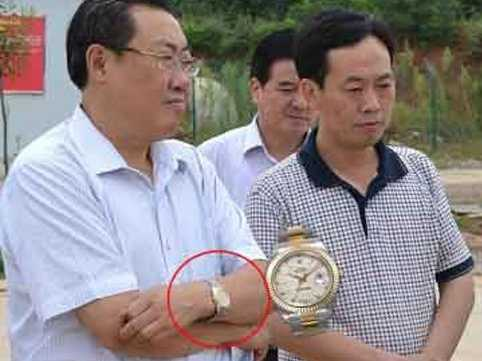
\includegraphics[scale=.4]{figures/annexes/biaoge/chinese-official-photographed-smirking-after-a-traffic-accident-that-left-36-dead-has-been-fired.jpg}}
    \newline
    \subfloat[]{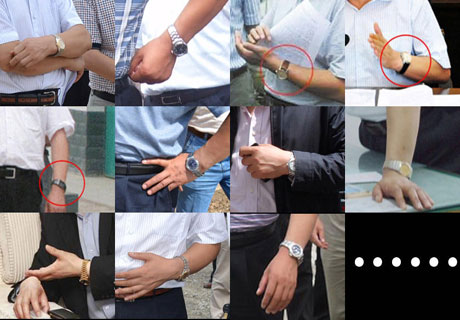
\includegraphics[scale=.5]{figures/annexes/biaoge/201209120198.jpg}}
    \subfloat[]{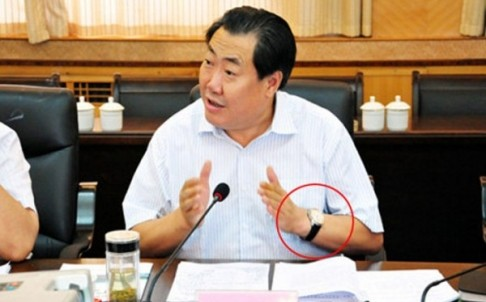
\includegraphics[scale=.5]{figures/annexes/biaoge/yang-dacai.jpg}}
    \caption{
      Images du mème entourant les montres de Yang Dacai
    }
\end{figure}

\clearpage

\subsection*{Yuan Fang, qu'en penses tu?}

Un dialogue issu d'une série policière très prisée présente un couple de détectives enquêtant dans la Chine médiévale. La phrase ``Yuanfang, qu'en penses-tu'' (\zh{元芳,你怎么看?}) est devenue aussi célèbre que le \textit{``élémentaire''} de Sherlock Holmes au Dr. Watson. 

\begin{figure}[ht]
    \centering
    \subfloat[]{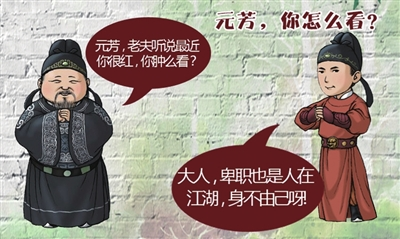
\includegraphics[scale=.4]{figures/annexes/yuanfang/50fa21e4d4994.jpg}}
    \subfloat[]{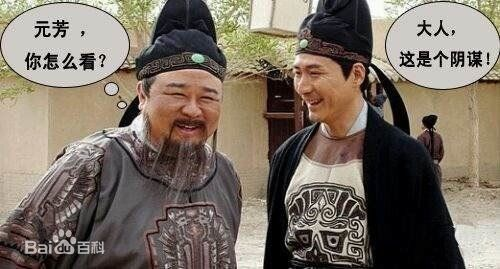
\includegraphics[scale=.6]{figures/annexes/yuanfang/960a304e251f95ca67b3a568c9177f3e660952ad.jpg}}
    \newline
    \subfloat[]{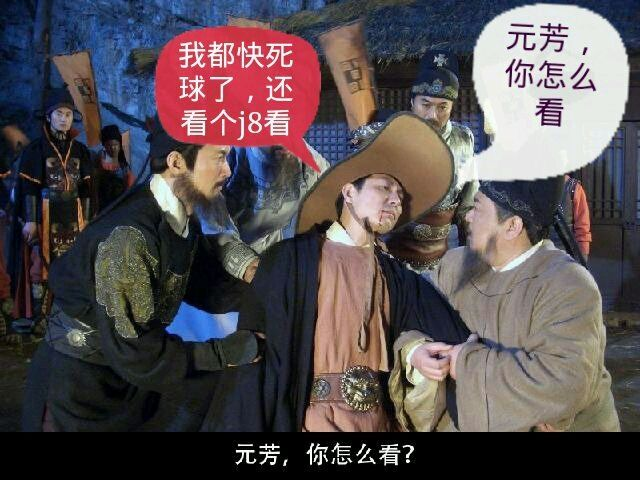
\includegraphics[scale=.3]{figures/annexes/yuanfang/2012102210340971752.jpg}}
    \subfloat[]{
\includegraphics[scale=.3]{figures/annexes/yuanfang/d4f21080968f3187.png}}
    \newline
    \subfloat[]{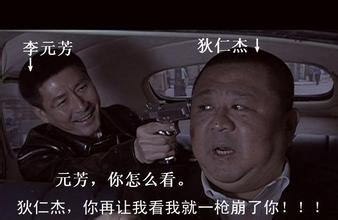
\includegraphics[scale=.5]{figures/annexes/yuanfang/u=4077910649,4163896412&fm=21&gp=0.jpg}}
    \subfloat[]{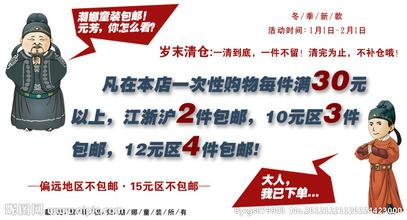
\includegraphics[scale=.5]{figures/annexes/yuanfang/ad.jpg}}
    \caption{
      Exemples d'images du mème \textit{Yuanfang}
    }
\end{figure}

\clearpage
\subsection*{Moyan}

Mo Yan (1955-) (en chinois \zh{莫言}) littéralement : « celui qui ne parle pas ») est un écrivain chinois célèbre. Le 11 octobre 2012, il a reçu le prix Nobel de littérature. Lors d'une interview sur une grande chaîne de télévision, il déclare ne pas pouvoir être heureux, trop stressé par sa récente réussite et par l'inquiétude que lui procure les changements de la Chine. Cette déclaration provoque rires, jalousies et moqueries sur la Toile.

Voir sa page sur Wikipedia \url{http://fr.wikipedia.org/wiki/Mo_Yan}


\begin{figure}[h!]
    \centering
    \subfloat[La cérémonie du Prix Nobel de Littérature]{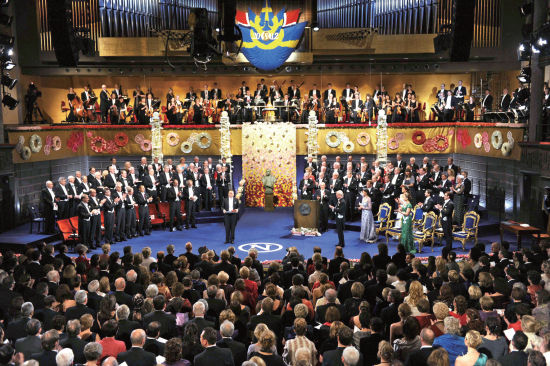
\includegraphics[scale=.42]{figures/annexes/moyan/U3875P843DT20121212080934.jpg}}
    \subfloat[Moyan répondant ``Je ne sais pas'' à la question ``Êtes-vous heureux ?'' par lors d'une interview sur la chaîne CCTV13]{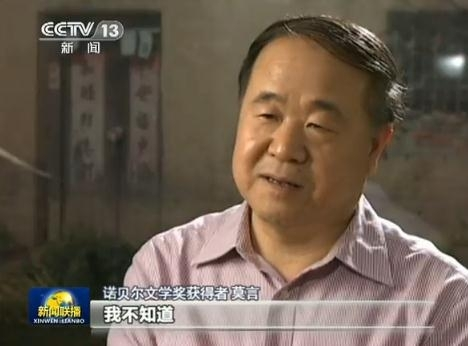
\includegraphics[scale=.45]{figures/annexes/moyan/1350256803891.jpg}}
    \newline
    \subfloat[Dessin d'un internaute moquant Mo Yan ``Je ne sais pas laquelle choisir'', d'après IT Times, \url{http://www.ittime.com.cn/index.php?m=content&c=index&a=show&catid=23&id=2662}, consulté le 7 Juillet à 14:32]{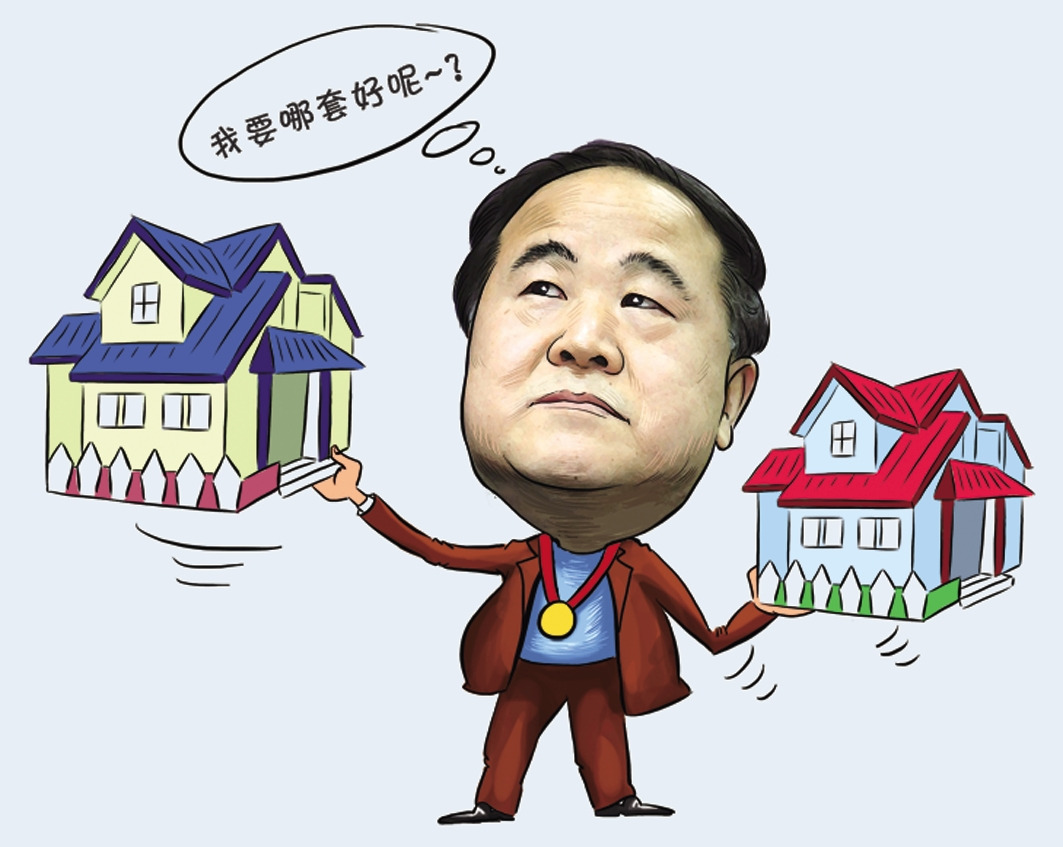
\includegraphics[scale=.8]{figures/annexes/moyan/20121112053840357.jpg}}
    \subfloat[Un dessin posté par un utilisateur de Sina Weibo]{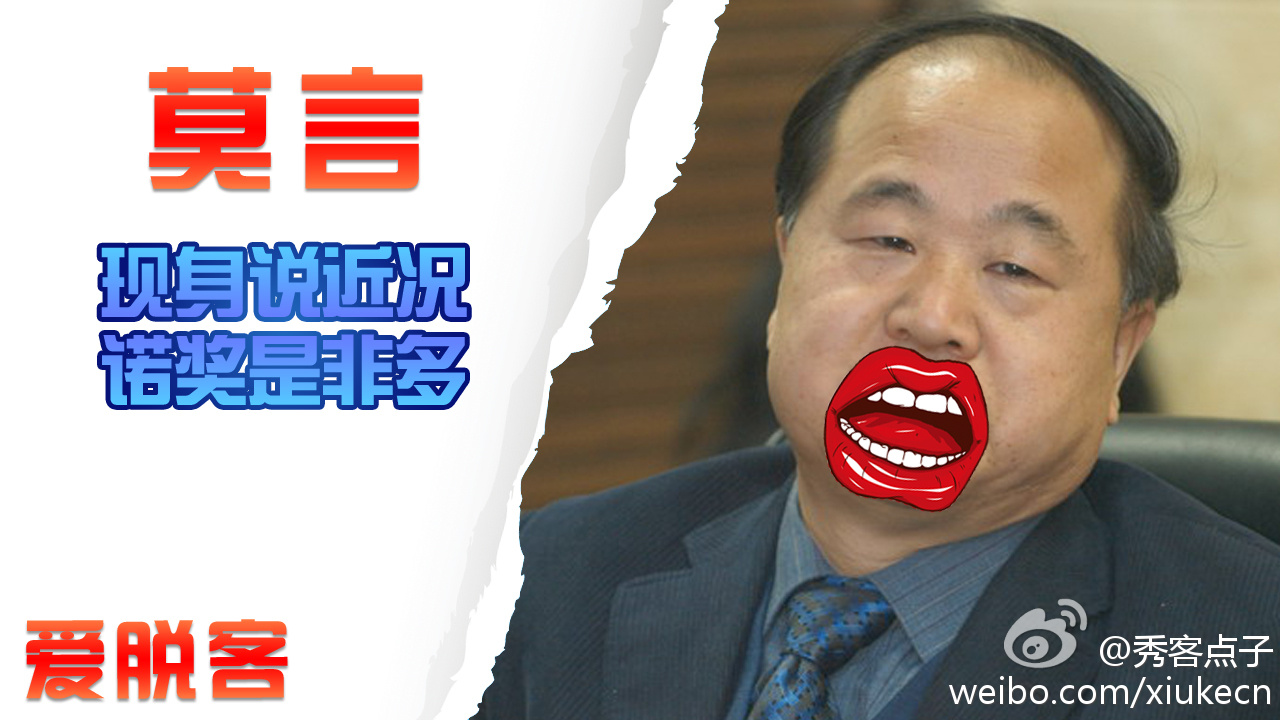
\includegraphics[scale=.2]{figures/annexes/moyan/a7be97b7jw1e1iic0yyb4j.jpg}}
    \caption{
      Mo Yan Prix Nobel : Illustrations
    }
\end{figure}

\clearpage
\subsection*{18ème Congrès du Parti Communiste}

Le XVIIIe congrès national du Parti communiste chinois (en chinois \zh{中国共产党第十八次全国代表大会}) s'est tenu en novembre 2012. Réunissant plus de 2270 délégués, ce congrès a élu Xi Jinping, l'actuel président chinois. La couverture médiatique de cet évènement majeur de la vie politique chinois en a fait un des temps forts de l'année 2012 dans les médias.

\begin{figure}[h!]
    \centering
    \subfloat[Le siège du 18ème Congrès du Parti Communiste à Pékin]{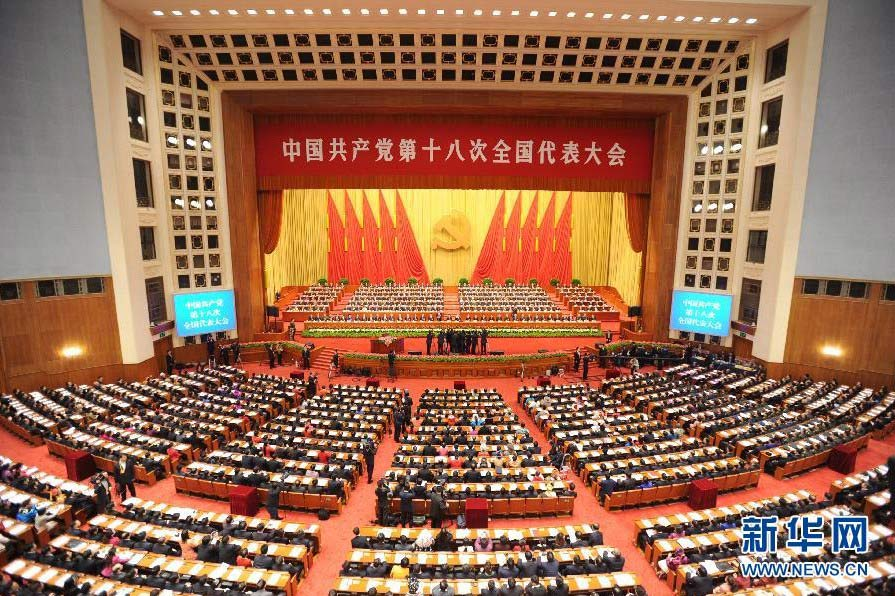
\includegraphics[scale=.17]{figures/annexes/CCP/147728760.jpg}}
    \subfloat[L'ancien président chinois Hu Jintao (à gauche) avec son successeur Xi Jinping (à droite)]{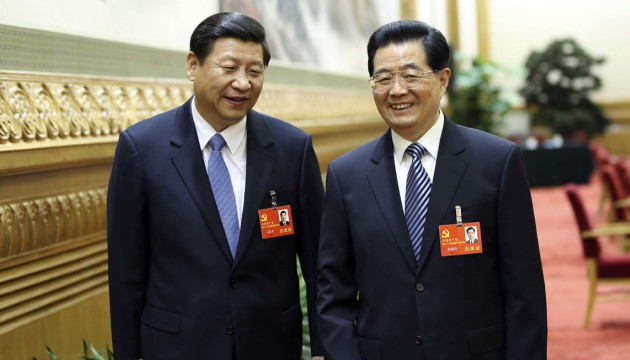
\includegraphics[scale=.3]{figures/annexes/CCP/4041352374032.jpg}}
    \newline
    \subfloat[Post bloqués lors de la recherche ``18ème Congrés'' sur Sina Weibo, d'après Feichang Dao, \url{http://blog.feichangdao.com/2012/11/in-week-before-party-congress-sina.html}, consulté le 27 Juillet à 16:53]{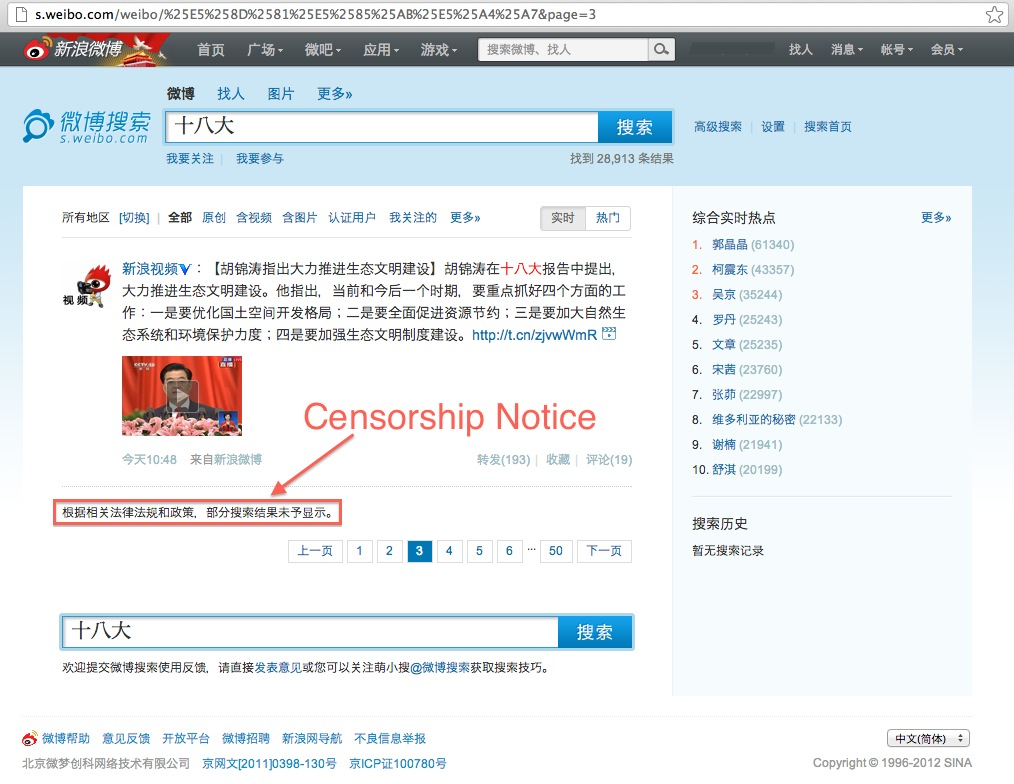
\includegraphics[scale=.4]{figures/annexes/CCP/18thCongress-18Big-SinaWeiboPage3-20121108-Annotated.jpeg}}
    \caption{
      18ème Congrès du Parti Communiste : Illustrations
    }
\end{figure}


\clearpage
\subsection*{Sex Tape}
\label{sec:sextape}

Une vidéo montrant Lei Zhengfu, le secrétaire du Parti dans le district de Beibei à Chongqing, dans le plus simple appareil en compagnie d'une de ses maîtresses est publiée en ligne. A peine 63h après la publication de cette vidéo avec le titre ``Lei, the secretary who accepts sex bribes'', Lei est mis à pied de ses fonctions politiques. Cette vidéo qui avait été tournée 4 ans auparavant été utilisée depuis plusieurs années par un promoteur immobilier de la ville de Chongqing pour faire chanter Lei Zhengfu. 

Voir aussi :
\url{http://en.wikipedia.org/wiki/Lei_Zhengfu}
et 
\url{http://www.viddler.com/v/41bf67b2}, consulté le 7 Juillet à 12:32

\begin{figure}[h!]
    \centering
    \hfill
    \subfloat[Image tirée de la vidéo]{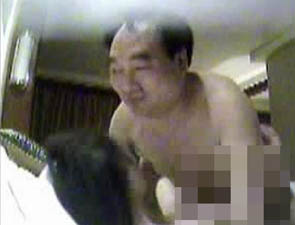
\includegraphics[scale=.8]{figures/annexes/sextape/Lei-Zhengfu.jpg}}
    \hfill
    \subfloat[Photo de la femme]{
\includegraphics[scale=.3]{figures/annexes/sextape/Lei-Zhengfu-Tape-Scandal-Leads-To-Chinese-Officials-Firing7.jpg}}
    \hfill
    \newline
    \hfill
    \subfloat[Détournement d'un internaute]{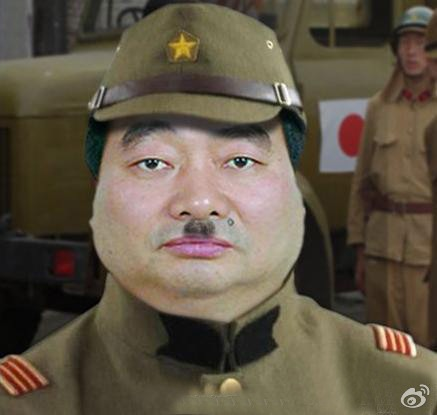
\includegraphics[scale=.5]{figures/annexes/sextape/lei05.jpg}}
    \hfill
    \subfloat[Détournement d'un internaute]{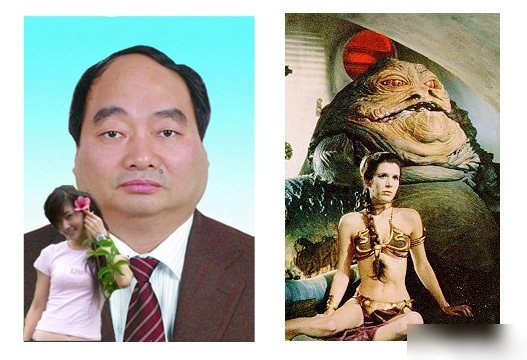
\includegraphics[scale=1.3]{figures/annexes/sextape/LeiJabba.jpg}}
    \hfill
    \caption{
      Exemples d'image du mème concernant la sextape de Lei Zhengfu. Images d'après l'article ``Sex tape official stands trial in Chongqing'' dans le \textit{People's Daily}, \url{http://english.peopledaily.com.cn/90882/8290628.html} et \url{http://www.dailymail.co.uk/news/article-2239300/Zhao-Hongxia-Teenage-honeytrap-brought-Chinese-Communist-Party-official-sex-tape-pictures-leaked-online.html} consulté le 7 Juillet à 12:32
    }
\end{figure}


\clearpage
\subsection*{Qiegao}

Qiegao (\zh{切糕}) est une gâteau au sucre et aux noix, spécialité de la région du Xinjiang souvent vendus par des vendeurs itinérants. Le 3 décembre 2012, une dispute entre un client villageois du Hunan et un vendeur  originaire de l’extrême-ouest de la Chine a tourné en altercation, avant de dégénérer en bagarre générale. Selon la police, le montant total des gâteaux abîmés a été estimé par la police à 160 000 yuans (environ 19 500€). Les internautes se sont emparés de cette affaire pour en faire une plaisanterie, comparant la valeur du Qiegao à celle de l’or.

Voir également \url{http://world.time.com/2012/12/05/dont-let-them-eat-cake-how-ethnic-tensions-in-china-explode-on-the-streets/} ou \url{http://chine.blogs.rfi.fr/article/2012/12/05/hans-ouighours-c-est-pas-du-gateau}


\begin{figure}[h!]
    \centering
    \subfloat[Un vendeur de qiegao]{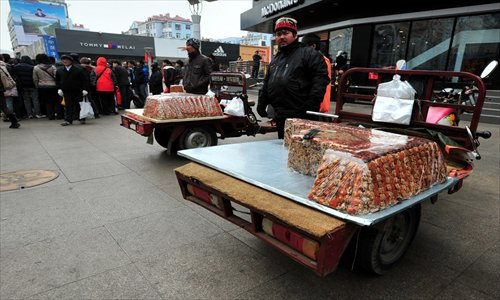
\includegraphics[scale=.65]{figures/annexes/qiegao/91914349-4fce-4373-b7dc-9fe05a0a28bf.jpeg}}
    \subfloat[Le gâteau]{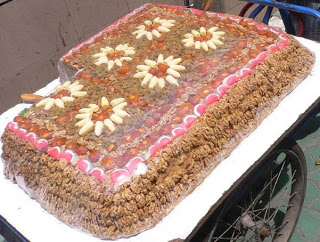
\includegraphics[scale=.7]{figures/annexes/qiegao/Qie-Gao.jpeg}}
    \newline
    \subfloat[Une image de l'affrontement avec la police posté par un utilisateur de Sina Weibo]{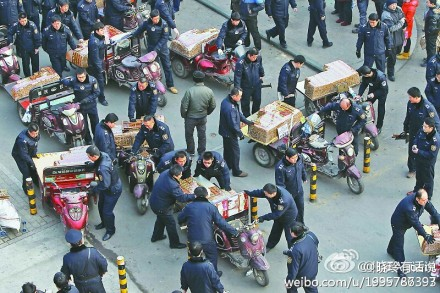
\includegraphics[scale=.65]{figures/annexes/qiegao/1.jpg}}
    \subfloat[Création d'un internaute montrant combien le qiegao est cher]{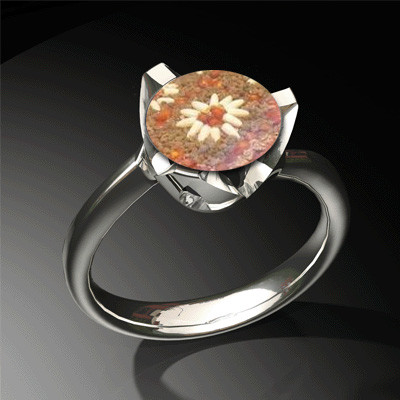
\includegraphics[scale=.66]{figures/annexes/qiegao/2.jpg}}
    \caption{
      Qiegao
    }
\end{figure}
